%%%%%%%%%%%%%%%%%%%%%%%%%%%%%%%%%%%%%%%%%%%%%%%%%%%%%%%%%%%%%%%%%%%%%%
% Problem statement
\begin{statement}[
  problempoints=100,
  timelimit=1 sekunda,
  memorylimit=512 MiB,
]{Semafor}

Vjerojatno ste se više puta u životu susreli sa tzv.\ \textit{7-segmentnim}
displejom koji se koristi za prikaz znamenaka na raznim digitalnim uređajima
poput satova ili kalkulatora. Zbog svoje jednostavnosti, intuitivnosti i
estetske ugode, takav je dizajn prihvaćen diljem planete.  Ipak, mladi Matej
smatra ga \textit{polu-proizvodom} te tvrdi da se ista funkcionalnost može
ostvariti na mnogo efikasniji način, koristeći svega pet segmenata.

\begin{figure}[H]
  \begin{center}
    
\includegraphics[width=0.8\textwidth]{img/5segment.png}

    \vspace{0.5cm}

    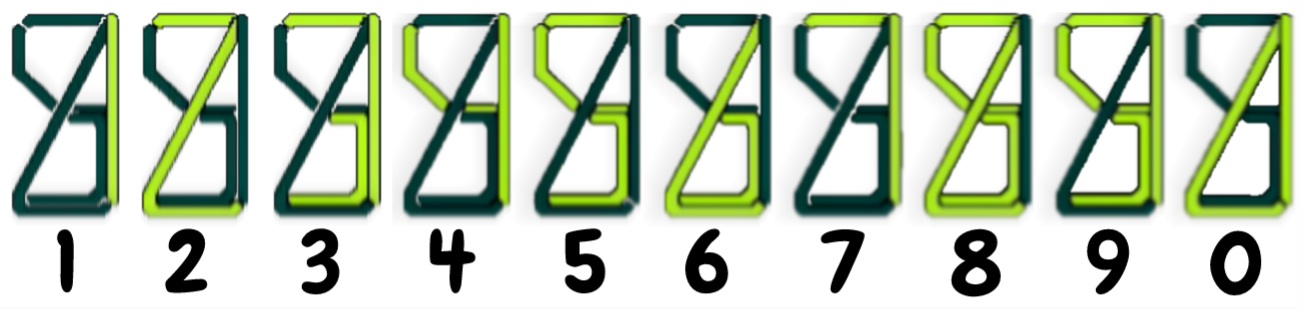
\includegraphics[width=0.8\textwidth]{img/5segmentdigits.png}
    \caption*{Dizajn 5-segmentnog displeja -- segmenti su označeni slovima od \texttt{a} do \texttt{e}.}
  \end{center}
\end{figure}
  \vspace{-0.7cm}
Prvi poduzetnički korak odlučio je napraviti u najprosperitetnijoj grani
hrvatske industrije -- nogometu. Svoj revolucionarni dizajn iskoristit će pri
izradi semafora za izmjene igrača tijekom utakmica 1.\ HNL, a trenutno radi
na prezentaciji koju će iznijeti čelnicima Hrvatskog nogometnog saveza.
Semafor se sastoji od $M$ displeja koji (slijeva nadesno) predstavljaju
znamenke broja kojeg nosi nogometaš koji treba izaći, odnosno ući u teren.
Na početku Matejeve prezentacije na semaforu će se nalaziti broj $X$, a Matej
će svake sekunde napraviti jedan od sljedećih poteza:
  \begin{itemize}
      \item Upalit će neki od ugašenih segmenata.
      \item Ugasit će neki od upaljenih segmenata.
  \end{itemize}
Također, Matej će pritom osigurati da se nakon svakog $K$-tog poteza na semaforu
nalazi ispravno napisan broj. Ukupno će Matej napraviti $N$ poteza, a na kraju
prezentacije (nakon $N$-tog poteza) semafor će također predstavljati ispravno
napisan broj. Broj je ispravno napisan ako je svaka njegova znamenka ispravno
napisana (kako je prikazano na slici). Također, brojevi koji imaju manje od
$M$ znamenaka trebaju sadržavati odgovarajući broj početnih nula.

Za svako završno stanje (cijeli broj između $0$ i $10^M-1$), Mateja zanima na
koliko je različitih načina mogao vući poteze da se na kraju prezentacije na
semaforu nalazi upravo taj broj te da su pritom zadovoljeni svi uvjeti iz
prethodnog odlomka. Dva načina (niza poteza) smatramo različitima ako, kada
bismo poteze istovremeno vukli na dva semafora, postoji trenutak u kojem
semafori ne prikazuju identično stanje. Budući da broj načina može biti
poprilično velik, potrebno je ispisati njegov ostatak pri dijeljenju s $10^9+7$.
%%%%%%%%%%%%%%%%%%%%%%%%%%%%%%%%%%%%%%%%%%%%%%%%%%%%%%%%%%%%%%%%%%%%%%
% Input
\subsection*{Ulazni podaci}
U prvom su retku prirodni brojevi $M$, $N$, $K$ $(1 \le K \le N)$ i $X$ $(0
\le X < 10^M)$ iz teksta zadatka.

%%%%%%%%%%%%%%%%%%%%%%%%%%%%%%%%%%%%%%%%%%%%%%%%%%%%%%%%%%%%%%%%%%%%%%
% Output
\subsection*{Izlazni podaci}
U $i$-tom od $10^M$ redaka izlaza treba se nalaziti broj različitih načina da
semafor na kraju prezentacije prikazuje broj $i-1$. Brojeve treba ispisati
modulo $10^9 + 7$.

%%%%%%%%%%%%%%%%%%%%%%%%%%%%%%%%%%%%%%%%%%%%%%%%%%%%%%%%%%%%%%%%%%%%%%
% Scoring
\subsection*{Bodovanje}
{\renewcommand{\arraystretch}{1.4}
  \setlength{\tabcolsep}{6pt}
  \begin{tabular}{ccl}
 Podzadatak & Broj bodova & Ograničenja \\ \midrule
  1 & 6 & $M=1$, $1 \le N \le 12$ \\
  2 & 9 & $M=1$, $1 \le N \le 10^{15}$ \\
  3 & 7 & $M=2$, $1 \le N \le 1500$, $K = N$\\
  4 & 21 & $M=2$, $1 \le N \le 10^{15}$, $1 \le K \le 15$ \\
  5 & 57 & $M=2$, $1 \le N \le 10^{15}$ \\
\end{tabular}}

%%%%%%%%%%%%%%%%%%%%%%%%%%%%%%%%%%%%%%%%%%%%%%%%%%%%%%%%%%%%%%%%%%%%%%
% Examples
\subsection*{Probni primjeri}
\begin{tabularx}{\textwidth}{X'X'X}
\sampleinputs{test/paint.dummy.in.1}{test/paint.dummy.out.1} &
\sampleinputs{test/paint.dummy.in.2}{test/paint.dummy.out.2} &
\sampleinputs{test/paint.dummy.in.3}{test/paint.dummy.out.3}
\end{tabularx}

%%%%%%%%%%%%%%%%%%%%%%%%%%%%%%%%%%%%%%%%%%%%%%%%%%%%%%%%%%%%%%%%%%%%%%
% We're done
\end{statement}

%%% Local Variables:
%%% mode: latex
%%% mode: flyspell
%%% ispell-local-dictionary: "croatian"
%%% TeX-master: "../hio.tex"
%%% End:
